% Homework template for Algorithm Analysis and Design
% UPDATE: September 20, 2019 by Xu Rongchen
\documentclass[a4paper]{article}
\usepackage{ctex}
\ctexset{
proofname = \heiti{证明} %% set proof name
}
\usepackage{amsmath, amssymb, amsthm}
% amsmath: equation*, amssymb: mathbb, amsthm: proof
\usepackage{moreenum}
\usepackage{mathtools}
\usepackage{url}
\usepackage{bm}
\usepackage{enumitem}
\usepackage{graphicx}
\usepackage{subcaption}
\usepackage{booktabs} % toprule
\usepackage[mathcal]{eucal}

\usepackage{iidef} % set homework count
\usepackage{longtable}

% \usepackage[noend]{algpseudocode}
\usepackage{clrscode3e}

\thecoursename{算法分析与设计实验报告}
\theterm{2019年秋季学期}
\hwname{排序算法比较}
\slname{\heiti{解}}
\begin{document}
\courseheader
\theusername{徐荣琛}
\thestuno{2019214518}
\theinstitute{软件学院}

\info

\begin{enumerate}
  \setlength{\itemsep}{3\parskip}
  %% Homework Start here:
  %% \item to enumerate the problem ID: Format as 'HomeworkID.ProblemID'
  %% \begin{solution} XXXX \end{solution} is to make a solution
  %% \begin{proof} XXXX \end{proof} is to make a proof
  %% Suggest to use \input{path} command
  \textbf{1.实验要求}\\
  比较insertionsort,shellsort,quicksort,mergesort以及radixsort对32位无
  符号整数的排序效果,要求给出一个实验报告。输入数据随机产生,数据范围为[0,$2^{32}-1$],
  输入数据量分别为:$10$,$10^2$,$10^3$,$10^4$,$10^5$,$10^6$,$10^7$,$10^8$,
  $2\times10^8$,($10^9$,此数量级选做)。\\
  \bigskip

  \textbf{2.实验环境}\\
  为了提高代码运行效率,此次实验代码采用C++语言实现,具体的实验环境及编译配置如下表所示:\\ \medskip
  \begin{tabular}{c|c}
    \hline\hline
    处理器 & Intel(R) Core(TM) i7-8850H CPU @ 2.60GHz \\ \hline
    内存 & 16GB\\ \hline
    操作系统& Mac OS X 10.14.6\\ \hline
    CMake版本& 3.14.1\\ \hline
    编译器& clang 11.0.0(C++14)\\ \hline
    Release编译参数& -O3\\
    \hline\hline
  \end{tabular}\\
  \bigskip

  \textbf{3.实验内容}\\
  \textbf{3.1 有关算法的实现}\\
  \medskip
  3.1.1 Insertion Sort:\\
  从数组第二个元素开始,逐一和前项比较,如果比前项小,则继续向前比较,否则停止这个元素的
  比较,并进入下一元素;\\
  \medskip
  3.1.2 Shell Sort:\\
  Shell Sort采用一个递减间隔序列$D$(最终为1),对于$D$中每一项$d_i$,对数组中每个距离
  $d_i$的子序列进行Insertion Sort。由于最终的间隔为1,保证了最后结果一定有序;\\
  \medskip
  3.1.3 Quick Sort:\\
  Quick Sort采用分治策略,先从数组中选择一个数作为划分依据,随后将所有数按和划分依据的大小关系
  进行分离,保证比划分依据小的数均在划分依据前,大的均在划分依据之后,随后对前后两部分继续递归;\\
  \medskip
  3.1.4 Merge Sort:\\
  Merge Sort亦采用分治策略,首先将数组分为等长的两部分(或长度差为1),对两部部分递归排序,直至
  仅剩一个元素,随后可在线性时间内对有序的两部分进行合并。合并时需要使用$O(n)$的辅助空间;\\
  \medskip
  3.1.5 Radix Sort:\\
  Radix Sort的基数为$R$的情况下,将待排序数表示为$R$进制:$a_0R^0+a_1R^1+a_2R^2+\cdots$,则
  依次对$a_0,a_1,a_2,\cdots$进行Counting Sort。Counting Sort需要使用$O(n)$的辅助空间;\\
  \medskip
  3.1.6 32位随机数生成:\\
  某些平台和C++标准下不能直接生成32位数,可随机出两个16位数,将一个左移16位异或上第二个即可。\\
  \medskip
  \textbf{3.2 部分排序算法的优化}\\
  \medskip
  3.2.1 Shell Sort:\\
  Shell Sort采用的间隔序列最初是采用$n/2,n/4,\cdots$,后经过相关资料查询,发现一个能够表现更优的序列:
  $a(n) = 9*2^n - 9*2^(n/2) + 1$($n$是偶数),$a(n) = 8*2^n - 6*2^((n+1)/2) + 1$($n$是奇数)。
  实验结果表明,在处理$10^8$数量级的排序数时,原先方法的耗时在26秒左右,优化方法的耗时在16秒左右,
  性能提升比例约38.5\%。\\
  \medskip
  3.2.2 Radix Sort:\\
  考虑到计算机实际结构,基数采用2的幂时应当具备更加的性能。在此基础上,对于一个数获取其对应的Count数组
  下标的方式采用二进制位运算,先将数右移需要的位数,再与上对于的二进制掩码$2^r-1$,即可获得数组下标。
  对于基数的大小,经过反复实验,发现在一定数据规模之上,$r=8$时有最佳的性能表现。\\
  % 3.2.2 Radix Sort:\\
  % Radix Sort采用链表存储作为桶的数据结构,但是实际运行速度较慢,分析其原因可能有两部分组成:\\
  % (1)链式存储的方式使得访存不连续,可能使得每次访问均需要请求内存,而不能从Cache中获得;\\
  % (2)简单的链式存储,每将一个32位数据串联均需要一个额外的64位地址空间,使得需要的初始化内存
  % 较实际扩大3倍,在内存申请和释放时效率降低(同时,同样大小下,非连续空间的内存申请和释放也较
  % 连续空间效率低)。\\
  % 于是优化了桶的数据结构,从简单的链表改为使用块状链表,初始化块大小为$1.01\times\frac{n}{m}$,
  % 增量块大小为$\max(\sqrt{\frac{n}{m}},1)$,其中$n$是数的个数,$m$是桶数。在随机分布的情况下,
  % 初始化块大小保证大多数块不需要再额外附加空间,增量块大小又保证了每次附加空间不显著增加空间消耗。
  % 同时\\
  \medskip
  \textbf{3.3 不同规模下的求解实验}\\
  \medskip
  随机生成的点人为要求其服从均匀分布,由于点的横纵坐标采用浮点数表示,所以希望得到在某一上下界内均匀
  分布的随即浮点数。.Net Core中$Rand$类提供了$NextDouble()$的方法随机出(0,1)范围内均匀分布的浮点
  数,故采用如下方式得到(LowerBound,UpperBound)范围内均匀分布的浮点数:
  $$NextDouble()*(UpperBound-LowerBound)+LowerBound$$\\
  设定上下界范围为(-100,100),随机1,000,000个点并执行最近点对算法,可以得到以下运行结果:
  \bigskip
  \begin{center}
    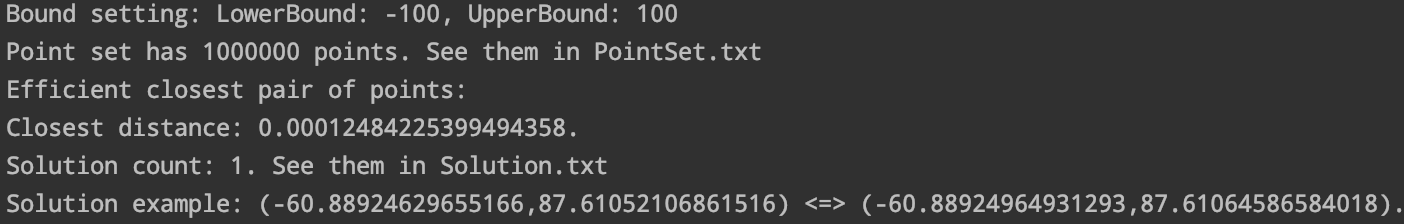
\includegraphics[scale=0.4]{Pictures/log.png}
  \end{center}
  此实验表明算法可以解决一百万个点规模的最近点对问题。\\
  \medskip
  \textbf{3.4 $\Theta(n^2)$和$\Theta(n\lg n)$算法在不同规模随机数据下的对比实验}\\
  \medskip
  3.4.1 实验概要:\\
  对于两种算法,分别随机产生出3组1E2, 5E2, 1E3, 5E3, 1E4, 5E4, 1E5, 5E5, 1E6数据规模的随机点,
  并在这些点集上进行对比实验,设置每组的超时时间为60秒。实验程序编译时设定为Release。\\
  \medskip
  3.4.2 实验结果:\\
  实验结果如下表所示:\\ \medskip
  \resizebox{\linewidth}{!}{ 
  \begin{tabular}{c||ccc|c||ccc|c}
    \hline\hline
    规模& $E1$& $E2$& $E3$& $EA$& $N1$& $N2$& $N3$& $NA$\\ \hline
    1E2&0.00894 &0.00160 &0.00092 &0.00382 &0.00118 &0.00033 &0.00012 &0.00054\\
    5E2&0.00341 &0.00383 &0.00234 &0.00319 &0.00104 &0.00123 &0.00125 &0.00117\\
    1E3&0.00498 &0.00484 &0.00482 &0.00488 &0.00372 &0.00388 &0.00390 &0.00383\\
    5E3&0.01946 &0.02137 &0.02123 &0.02069 &0.06167 &0.06072 &0.05958 &0.06066\\
    1E4&0.04915 &0.04257 &0.04194 &0.04455 &0.19470 &0.18785 &0.19036 &0.19097\\
    5E4&0.20651 &0.21944 &0.22987 &0.21861 &4.23536 &4.23443 &4.49164 &4.32047\\
    1E5&0.63202 &0.41690 &0.40984 &0.48626 &17.51799 &17.18423 &17.14976 &17.28399 \\
    5E5&2.87273 &3.52119 &4.18541 &3.52644 &Timeout &Timeout &Timeout &Timeout\\
    1E6&10.46015 &12.58344 &14.94236 &12.66198  &Timeout &Timeout &Timeout &Timeout\\
    \hline\hline
  \end{tabular}
  }\\
  \medskip
  表中,$E1,E2,E3,N1,N2,N3$分别表示高效算法(Efficient)和暴力算法(Naive)三次实验的结果,$EA,NA$是三次实验的均值。
  时间单位为秒。\\
  \medskip
  3.4.3 实验分析:\\
  以数据规模为横坐标,算法耗时为纵坐标(为方便低数量级的展示,故这里采用对数坐标),绘制出如下的
  耗时曲线比较图:
  \begin{center}
    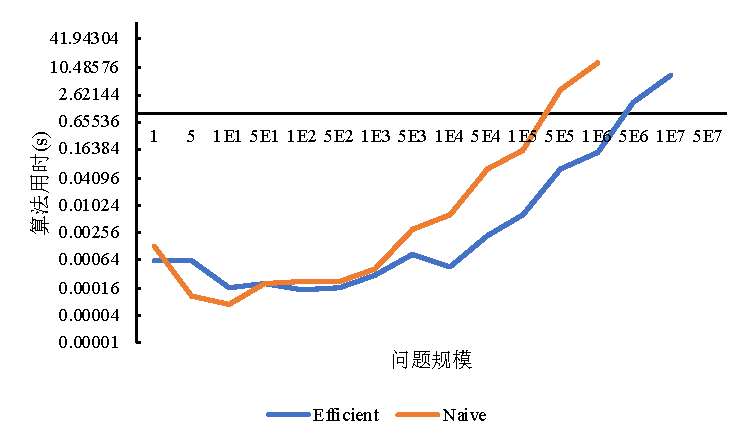
\includegraphics[scale=0.8]{Pictures/Chart.pdf}
  \end{center}
  从图中可发现,当数据规模小于$10^3$数量级时,暴力方法能够更快解决问题,当数据规模超过$10^3$数量级后,
  复杂度为$O(n \lg n)$的算法表现出了明显的计算优势。尤其是,面对5E5和1E6规模的问题时,暴力算法已经不
  能在1分钟内进行求解。\\
  有趣的一点是$O(n \lg n)$的算法在1E2的平均耗时比5E2规模的平均耗时几乎一致(甚至略高),说明数据较小
  时,主要耗时并不由数据规模决定,而是由常数决定。\\
  另一方面,可以发现暴力方法的三次实验用时较$O(n \lg n)$算法更加趋于一致,说明暴力方法时间消耗更加稳定,
  而$O(n \lg n)$算法耗时可能取决于数据内容,这也与算法实现相吻合。
\end{enumerate}


\end{document}